% Define the module top matter
% This gets used to create the chapter title page
\setModuleTitle{Eukaryotic Assembly}
\setModuleAuthors{%
  Bernardo Clavijo, TGAC \mailto{Bernardo.Clavijo@tgac.ac.uk} \\
}
\setModuleContributions{%
  Sonika Tyagi, AGRF \mailto{sonika.tyagi@agrf.org.au}
  Zhiliang Chan \mailto{zhiliang@unsw.edu.au}
}

\chapter{\moduleTitle}
\newpage
% END: Module Title Page


\section{Key Learning Outcomes}

After completing this module the trainee should be able to:
\begin{itemize}
  \item Assess general assembly approach, kmer spectra and biases.
  \item visually inspect the kmer spectra and KAT plots
  \item run a first pass eukaryotic assembly and do goal checks 
  \item Develop validation metrics or tools for NGS data and assembly.
  \item Improving methods and pipelines for genome assembly.
  \item Convince the lab guys to tweak protocols.

\end{itemize}
% END KLOs

\section{Resources You'll be Using}
 
\subsection{Tools Used}
\begin{description}[style=multiline,labelindent=0cm,align=left,leftmargin=0.5cm]
  \item[Kmer Analysis Tool kit]\hfill\\
  	\url{https://github.com/TGAC/KAT}
  \item[Nextclip]\hfill\\
  	\url{https://github.com/richardmleggett/nextclip}
  \item[Abyss]\hfill\\
  	\url{http://www.bcgsc.ca/platform/bioinfo/software/abyss}
  \item[Soap Denovo]\hfill\\
  	\url{http://soap.genomics.org.cn/soapdenovo.html}
  \item[SOAPec]\hfill\\
  	\url{http://soap.genomics.org.cn/about.html}
\end{description}

\section{Data source}

%\begin{information}
%Information to be provided to the trainee.
%\end{information}

\newpage

% BEGIN: Introduction
\section{First Pass Genome Assembly}
\begin{information}
Assuming by now you are familiar with the general concept of \textit{de novo} assembly, kmers and the de Bruijn graph based assembler. In this tutorial we will use ABySS to perform  the first pass assembly of a eukaryotic genome and look at various parameters to assess the information content of the input data and choice of assembly parameters. 
sequence data. 
Genome assembly is a challenging problem requiring heavy computational resources, expertise and time. Before you beging the process of denovo assembly there are a number of points you need to consider:
\item What is the objective of your assembly experiment ? What biological question(s) you have ?
\item Is assembly strictly neccessary for the purpose in question ?
\item Do you have right kind of data and enough coverage to start with ?
\item Do you have suitable computaitonal resources to run this assembly ?

\end{information}

\begin{note}
Remember that the assembly is just a probabilistic model of a genome, condensing the information 
from the experimental evidence.  All the information is already present in the 
experimental results. The goal of the assembly is to find the right motifs, 
the correct number of times, in correct order and position.
\end{note}


\subsection{Fusarium first pass with a goal}

\begin{information}
Goal: test horizontal gene transfer of necrotrophic genes
\item Reference genome for \textit{F. graminareum} (non necrotrophic)
\item Reference genome for \textit{F. pseudograminareum} (necrotrophic)
\item Blast database of cereal pathogen proteins.
\item Strategy: to check proteins on the necrotrophic genome, present on the protein database and not present on the non-necrotrophic genome.
\item Assembly goal (I): to capture a good enough representation of the protein-coding space to get blast matches
\item Assembly goal (II): to accurately represent possible horizontal-transfer loci.


\end{information}

\section{Prepare the Environment}
\begin{steps}
Open the Terminal.
First, go to the right folder, where the data are stored.
\begin{lstlisting}
cd /home/trainee/euk_assem
ls
\end{lstlisting}
\end{steps}

\subsection{Task1.1: First pass assembly, k=71}

\begin{steps}
Let's assemble \textit{Fusarium} with abyss, k=71
\begin{lstlisting}
%%%%%%% CHECK THE PATH IN THE VM
cd ~/denovo/fusarium
mkdir abyss_k71
cd abyss_k71
abyss-pe in="../CS3270_A8733_GCCAAT_L001_R1.fastq ../CS3270_A8733_GCCAAT_L001_R2.fastq" k=27 name=CS3270_abyss_k71 np=4 > CS3270_abyss_k71.log 2>&1
\end{lstlisting}
\end{steps}

Description of the arguments used in the command:
\begin{description}[style=multiline,labelindent=0cm,align=right,leftmargin=\descriptionlabelspace,rightmargin=1.5cm,font=\ttfamily]
  \item[k] = kmer size
  \item[np] = number of processors to be used
  \item[sequence file names] = R1 and R2 reads of a paired end sequence data
\end{description}

\begin{steps}
Let's look at the statistics of the assembly we just did... 

Ok, there is no stats available in the folder, but we can always use \texttt{abyss-fac} to get the stats:
\begin{lstlisting}
abyss-fac CS3270_abyss_k71-*tigs.fa  | tee CS3270_abyss_k71-stats.tab
less CS3270_abyss_k71-stats.tab
\end{lstlisting}
\end{steps}


\begin{table}[H]
  \centering
  \caption{Statistics of fusarium assembly by ABySS using k=71}
    \begin{tabular}{rrrrrrrrrrr}
    \toprule
    \textbf{n} & \textbf{n:500} & \textbf{L50} & \textbf{min} & \textbf{N80}& \textbf{N50}& \textbf{N20}& \textbf{E-size}& \textbf{max} & \textbf{sum}& \textbf{name}\\
    \midrule
    27 & 13 & 2 & 970 & 6004 & 13202 & 52602 & 28712 & 52602 & 112849 & CS3270_abyss_k71-unitigs.fa\% \\
    5 & 1 & 1 & 128429 & 128429 & 128429 & 128429 & 128429 & 128429 & 128429 & CS3270_abyss_k71-contigs.fa\% \\
    \bottomrule
    \end{tabular}
  \label{tab:fusariumk71}
\end{table}


\begin{questions}
How many unitigs/contigs do you have in the assembly?
\begin{answer}
27/5
\end{answer}
What are the length statistics of your assembly?
\begin{answer}
in the table above
\end{answer}
Does it match what you think before the assembly and why?
\begin{answer}
No
\end{answer}

\end{questions}


\begin{steps}
The assembly is looking strange! It's time for some analysis:

\item Check frequencies for kmers kept/discarded/etc.
\item Check spectra-cn and compare with expectations.
Let's do this by the following commands:

\begin{lstlisting}
less CS3270_abyss_k71.log 
less coverage.hist
\end{lstlisting}
\end{steps}

\begin{steps}
We will now plot the values from the \texttt{coverage.hist}:
\begin{lstlisting}
gnuplot <Press enter>
%gnuplot> set xrange [0:50]
%gnuplot> set yrange [0:4000000]
%gnuplot> plot "coverage.hist"
%%%%%%% CHECK one of the plotting commands need to be deleted
%gnuplot
gnuplot> set xrange [0:200]
gnuplot> set yrange [0:5000]
gnuplot> plot "coverage.hist"
\end{lstlisting}
\end{steps}


\start{steps}
Let us generate k-mer spectra of this assembly:
\start{lstlisting}
kat comp -o reads_vs_abyss_k71 '../*.fastq' CS3270_abyss_k71-contigs.fa
kat plot spectra-cn -y 1000 -x 1000 -o reads_vs_abyss1-main.mx.spectra-cn_1000_1000.png reads_vs_abyss1-main.mx
\end{lstlisting}
\end{steps}

The kmer spectra for \textit{Fusarium} assembly with abyss, k=71 should be looking like this:
\begin{figure}[H]
\centering
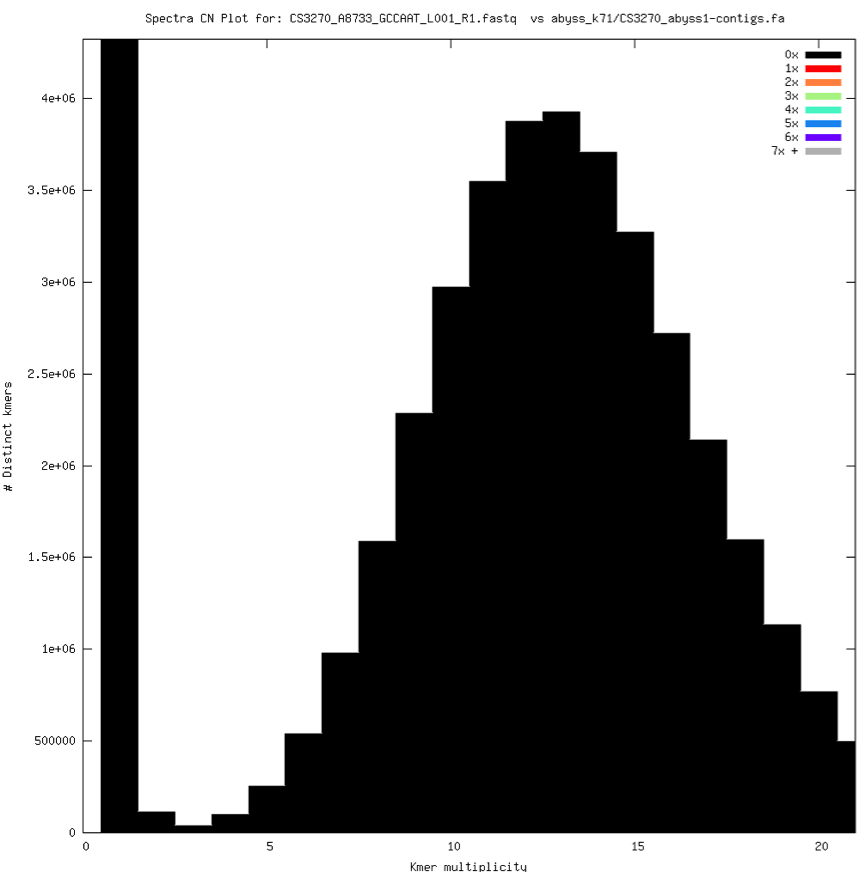
\includegraphics[width=0.8\textwidth]{handout/abyss-k71.png}
\caption{Kmer spectrum for \textit{Fusarium} assembly with abyss, k=71, coloured by the frequencies asfound on the reference assembly.}
\label{fig:fusariumk71}
\end{figure}

Take the output and BLAST it in NCBI. What is it? Surprising?

\begin{steps}
%Blast commands, May be pre-cooked
\end{steps}

Choosing a wrong k value (too large in this case) and just running a typical assembly job, we can end up with something quite more interesting. It is easy by comparison to spot some missing content, alongside duplications and triplications (and quadruplications and so on) that should not be there.
This assembly will get us nowhere, let's choose a lower K to gain coverage and start again.

\subsection{Task1.2: First pass assembly, k=71}
\begin{steps}
We now assemble \textit{fusarium} with \texttt{abyss} and k=27:
\begin{lstlisting}
cd ~/denovo/fusarium
mkdir abyss_k27
cd abyss_k27
abyss-pe in="../CS3270_A8733_GCCAAT_L001_R1.fastq ../CS3270_A8733_GCCAAT_L001_R2.fastq" k=27 name=CS3270_abyss_k27 np=4 > CS3270_abyss_k27.log 2>&1
\end{lstlisting}

\begin{steps}
Let's look at the stats by doing:
\begin{lstlisting}
less CS3270_abyss_k27-stats.tab
\end{lstlisting}
\end{steps}

Stats look better:
\begin{table}[H]
  \centering
  \caption{Statistics of fusarium assembly by ABySS using k=27}
    \begin{tabular}{rrrrrrrrrrr}
    \toprule
    \textbf{n} & \textbf{n:500} & \textbf{L50} & \textbf{min} & \textbf{N80}& \textbf{N50}& \textbf{N20}& \textbf{E-size}& \textbf{max} & \textbf{sum}& \textbf{name}\\
    \midrule
    30645  & 2717   & 430  & 502  & 11354   & 25336   & 47966    & 31027   & 147694   & 36.14e6  & CS3270_abyss_k27-unitigs.fa
	21511  & 350    & 33   & 527  & 157565  & 338989  & 630228   & 407098  & 1265237  & 36.52e6  & CS3270_abyss_k27-contigs.fa
	21327  & 205    & 17   & 527  & 332444  & 716132  & 1265237  & 791882  & 1880850  & 36.51e6  & CS3270_abyss_k27-scaffolds.fa
    \bottomrule
    \end{tabular}
  \label{tab:fusariumk27}
\end{table}


\begin{steps}
Let's check a bit anyway:
\begin{lstlisting}
less CS3270_abyss_k71.log
less coverage.hist
\end{lstlisting}
\end{steps}

\startend{steps}
How is the coverage plot looking now?
\start{lstlisting}
gnuplot
gnuplot> set xrange [0:50]
gnuplot> set xrange [0:4000000]
gnuplot> plot "coverage.hist"
%exit gnuplot

\end{lstlisting}
\end{steps}



\start{steps}
K-mer spectrum:
\startend{lstlisting}
kat plot spectra-cn -y 1000 -x 1000 -o reads_vs_abyss1-main.mx.spectra-cn_noabsent.png reads_vs_abyss1-main.mx
\end{lstlisting}
\end{steps}

\begin{figure}[H]
\centering
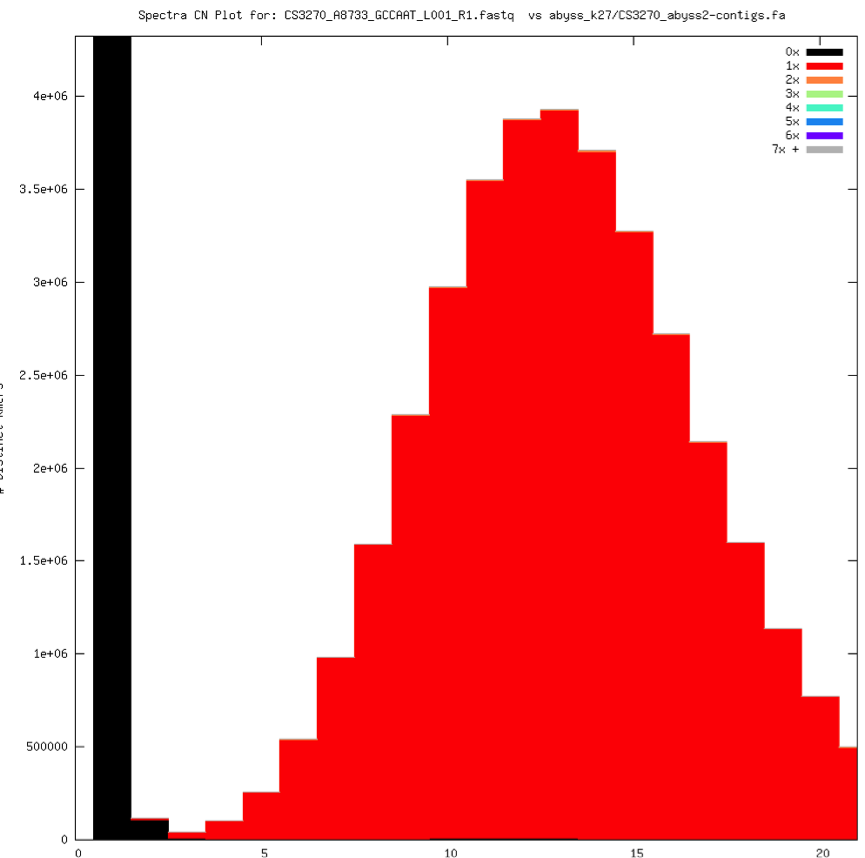
\includegraphics[width=0.8\textwidth]{handout/abyss-k27.png}
\caption{Kmer spectrum for \textit{Fusarium} assembly with abyss, k=27, coloured by the frequencies asfound on the reference assembly.}
\label{fig:fusariumk27}
\end{figure}


\begin{questions}
Any tools I can use to check kmer spectra at any K before assembling?
\begin{answer}
KAT
\end{answer}
\end{questions}

\begin{steps}
Will the assembly answer the biological question?

Use BLAST and the databases to check...
\end{steps}

